\section{Simplification of the Gluing Condition}
\label{A:gluing BC simplification}

The general form for the conservation of probability flux condition was given in equation~\eqref{E:cpfc}. The probability flux, $J$, is given in equation~\eqref{E:prob flux} and $\nu^n$ represents the outward normal vector of leaf $n$. $z = (h,i) = \mathcal{O}$ is used to denote the gluing vertex. In this appendix we show that the conservation of probability flux condition simplifies to equation~\eqref{E:cpfc simplified}.

The first step towards this simplification is to exploit the fact the gluing vertex is aligned with the $h=0$ axis, therefore equation~\eqref{E:cpfc} for the two-leaf autoparametric system becomes
\begin{equation}
\lim_{h \to 0} \left(J^1_1(h,i) - J^2_1(h,i)\right) = 0.
\label{E:cpfc intermediate}
\end{equation}
Next, individual terms of the probability flux must be considered. First we consider those simplifications that can be made analytically. From~\eqref{E:drift h}, it follows that $\mathring{\mathfrak{b}}_1^n = - (\zeta_o + 2\zeta_p) H \period_n$ (for $n=1,2$.) Since as $h \to 0$, the period is asymptotically equivalent to $\period(z) \sim \ln |H|$, the following results:
\[
\lim_{h \to 0} \mathring{\mathfrak{b}}_1^n = 0
\]
Similarly, from equation~\eqref{E:diffusion hi} it follows that $\mathring{\Aa}_{12}^n = \sigma^2 S_{\xi\xi}(1) H \period_n$. Again, the asymptotic behavior of $\period(z)$ yields:
\[
\lim_{h \to 0} \mathring{\mathfrak{a}}_{12}^n = 0
\]
The fact that $\mathring{\mathfrak{a}}_{11}^1 = \mathring{\mathfrak{a}}_{11}^1 = \sigma^2 S_{\xi\xi}(1) I \sqrt{I}/3$ (see equation~\eqref{E:lim drift_11}) is also used to simplify equation~\eqref{E:cpfc intermediate}.

The final two simplifications are
\begin{align*}
\lim_{h \to 0} \frac{\partial \mathring{\Aa}_{11}^n}{\partial h} &= 0,&
\lim_{h \to 0} \frac{\partial \mathring{\Aa}_{12}^n}{\partial i} &= 0
\end{align*}
for $n=1,2$. These two simplifications can be demonstrated numerically, as shown in Figures~\ref{F:lim a11} \& \ref{F:lim a12}.

\begin{figure}
\begin{center}
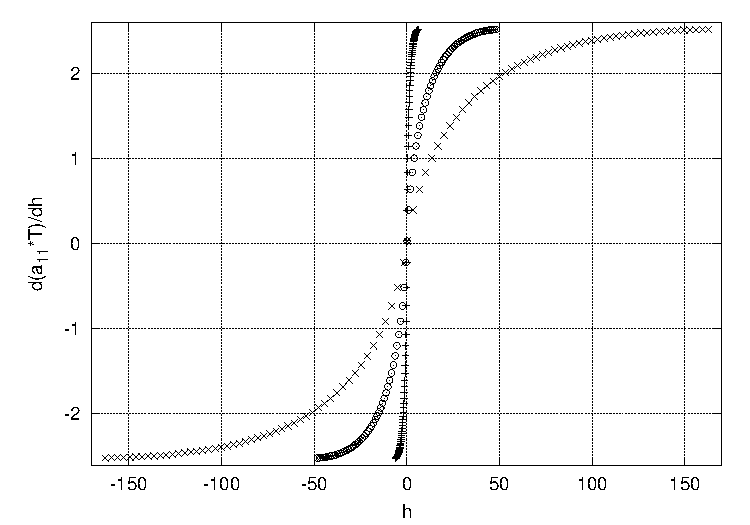
\includegraphics[width=\textwidth*7/8,angle=0]{figures/lim_a11}
\caption{Numerical demonstration that $\lim_{h \to 0} \frac{\partial\mathring{\Aa}_{11}^n}{\partial h} = 0$. Each dataset is for a different value of $i$.}
\label{F:lim a11}
\end{center}
\end{figure}

\begin{figure}
\begin{center}
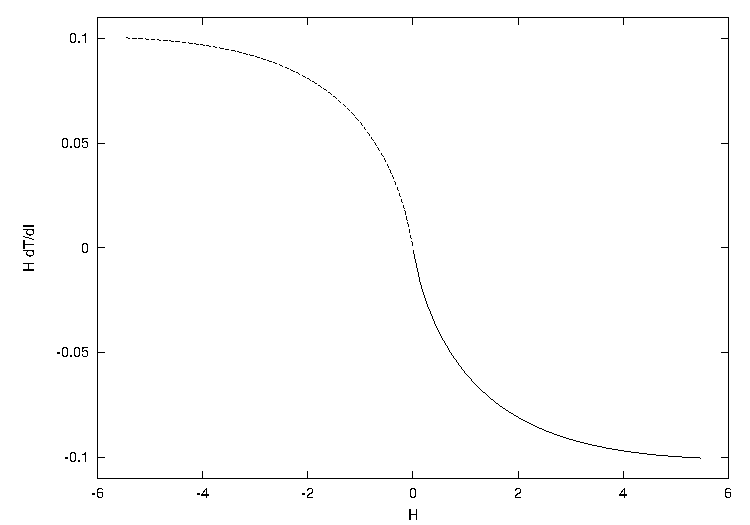
\includegraphics[width=\textwidth*7/8]{figures/cpfbc_numerical_demo}
\caption{Numerical demonstration that $\lim_{h \to 0} h \cdot d\period/di = 0$. This result demonstrates that $\partial \mathring{\Aa}_{12}/\partial I = 0$, that is used to simplify the conservation of probability flux condition.}
\label{F:lim a12}
\end{center}
\end{figure}

% Kludge to fix Figure numbering problem
\begin{figure}
\begin{center}
\label{F:lim a122}
\end{center}
\end{figure}

%% How might numerical simplifications be made analytic?
